\section{Results and Discussion}
\label{sec:results-and-discussion}

The validity of a reproducibility standard can only be established by regenerating an assessment from the record it prescribes, using no information beyond that contained in the record itself. The principal test of ORCHID-SAGE therefore consists of the independent regeneration of the Cr--Ni thermodynamic database from its specific protocol, and this test is presented before the assessment, since it constitutes the main evidence supporting the central claim of this work. Two independent regenerations were performed, one through scripted execution of the reproduction plan and one by an AI agent with access to the ORCHID-SAGE server tools and to read-only file tools, and in both cases the results were compared with those of the original assessment using the tolerances declared in the protocol (\cref{fig:verification}b).

\subsection{Reproduction of the Cr--Ni assessment}
\label{sec:reproduction}

The first regeneration was carried out with a script on an NVIDIA DGX Spark (aarch64, Linux), a machine that differs from the Mac Studio (arm64, macOS) used in the assessment in its processor, its operating system and its numerical libraries. Only the records files, identified by their SHA-256 hashes, were available on this machine. Of the 13 checks declared in the protocol, the five deterministic ones (the phases calculated at the 695 evaluated states, the phase sequence on heating at 99 compositions and the stable phases of the pure elements) gave identical results (\cref{fig:repro}). The eight numerical checks agreed within their tolerances, with a difference of $4 \times 10^{-9}$ in the objective (i.e. log likelihood) of the selected solution and no difference in the eutectic and CrNi$_2$-top temperatures (\cref{fig:verification}b). The selection rule picked a different start on this machine (s1 instead of s4), although both starts belong to the same posterior mode and lie 0.039 tolerances apart in parameter space. For this reason, the parameters are compared only as a note, while the model's predictions are compared within tolerances.

The second regeneration was carried out by an AI agent (Claude Opus 5.5), which had access to the tools of the ORCHID-SAGE server and to read-only file tools but received no information about the assessment other than the identifier of its specific protocol. Using only these tools, the agent read the protocol, staged its inputs, executed each of its steps through the server and compared the results to the recorded ones. This regeneration required 46 turns and 2~h~38~min, at a cost of US\$1.64 in model usage. Since it took place on the Mac Studio, the eight starts of the final step reproduced the original ones exactly, and all 13 checks were passed, eleven of them without any difference and the other two (the best results of basin hopping and dual annealing) with differences of the order of $10^{-12}$ in the objective. These (preliminary) results show that an AI agent can regenerate a CALPHAD database from its record alone, without human intervention, and this is precisely the condition a living database, updated every time new data appear, must satisfy. The same refit was finally repeated from a clean copy of the public repository of ORCHID-SAGE, in an environment built only from public sources (ESPEI, pycalphad and PhaseForge+ at their recorded commits), and the selected solution, the eutectic and the top of CrNi$_2$ were again reproduced exactly, in about one hour on a single workstation.

\begin{figure}[tbp]
    \centering
    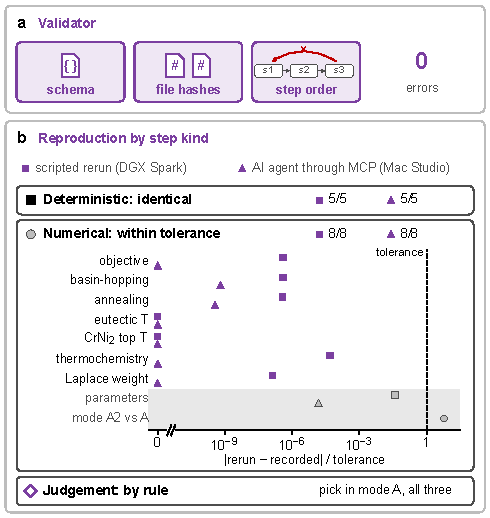
\includegraphics[width=83mm]{fig_verification_1col_1}
    \caption{Verification of the specific protocol and of its reruns. (a)~The validator checks that every document conforms to the schema, that every referenced file exists with its recorded hash and that no step uses an input before it is produced. (b)~Two independent reruns, one scripted on a DGX Spark and one by an AI agent through the ORCHID-SAGE server on the Mac Studio, compared with the original by step kind: deterministic outputs are identical, numerical outputs are shown relative to their declared tolerances, and the judgment step picks a start in the same mode in all three runs. The parameters are compared only as a note (grey).}
    \label{fig:verification}
\end{figure}

\begin{figure*}[tbp]
    \centering
    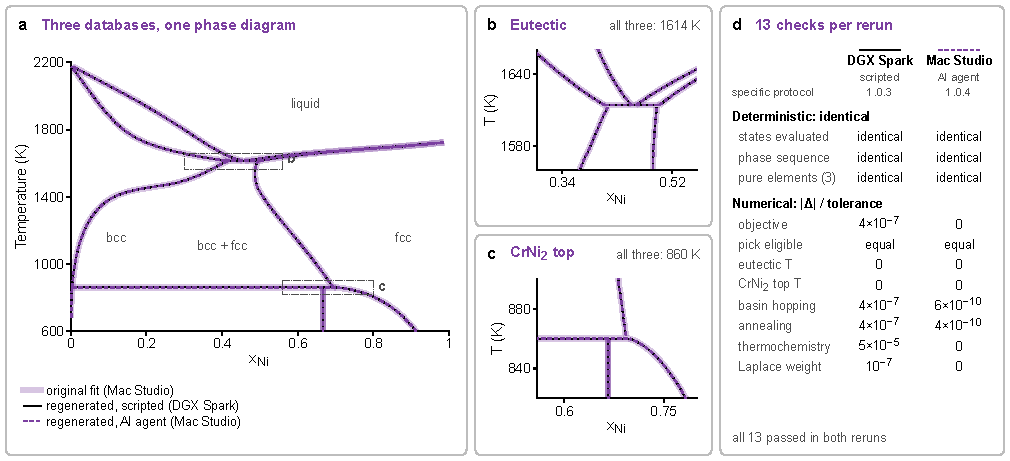
\includegraphics[width=171mm]{fig_hero_repro}
    \caption{Regeneration of the Cr--Ni database from its record. (a)~Phase diagrams calculated from the database of the original assessment (broad light purple line) and from the databases regenerated by the scripted rerun on a DGX Spark (black line) and by the AI agent on the Mac Studio (dashed purple line). (b)~The eutectic and (c)~the top of CrNi$_2$, enlarged, with the temperature given by all three databases. (d)~The checks of the specific protocol for each rerun: deterministic checks give identical results, and numerical checks are shown as the difference from the recorded value relative to its tolerance.}
    \label{fig:repro}
\end{figure*}

In the final step of the fit for the Cr--Ni system, the objective was observed to have two minima of almost the same value (modes A and A2 in \cref{fig:modes}), which differ by only 0.0045 log units but by up to 5.9 times the parameter tolerance in the first-order Redlich--Kister terms of bcc and fcc. On the original machine, seven of the eight starts converged to mode A and one to A2, while on the second machine the split was five to three. Both modes, however, give identical phase diagrams, invariant temperatures and thermochemical properties. The data used in the fit therefore do not determine these two terms within the declared tolerance, and they are reported as undetermined in the record. In a conventional assessment, in which a single set of parameters is published, this would most likely have gone unnoticed.

\begin{figure}[tbp]
    \centering
    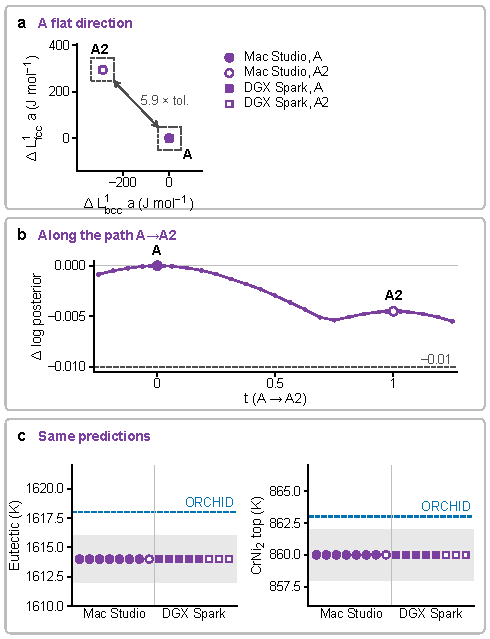
\includegraphics[width=83mm]{fig_verification_1col_2}
    \caption{Two modes of the final fit with the same predictions. (a)~The two minima of the basin, A and A2, in the plane of the bcc and fcc first-order terms, 5.9 times the parameter tolerance apart (dashed boxes). (b)~Log posterior along the straight path from A to A2, which stays within the tolerance of 0.01 on the objective (dashed). (c)~Eutectic and CrNi$_2$-top temperatures at every start (filled, mode A; open, A2) on both machines, within \qty{\pm 2}{\K} of the recorded values (grey), with the ORCHID records (dashed). ORCHID v2026.10 and records extracted for this work; record identifiers are provided with the source data.}
    \label{fig:modes}
\end{figure}

\subsection{Cr--Ni: the worked case}
\label{sec:crni}

As mentioned above, the assessment starts with the one-shot model of PhaseForge~\cite{zhu2025accelerating,zhu2025machinelearningpotentialsalloys}, which combines potential-calculated energetics with SGTE descriptions of the pure elements. Although this model contains all phases of the system, its phase diagram is displaced at high temperatures (\cref{fig:sequence}a), and this error can be traced back to a single end-member. Fcc Cr is mechanically unstable, and its energy relative to bcc Cr is \qty{7.3}{\kilo\joule\per\mole} in the SGTE description but about \qty{38}{\kilo\joule\per\mole} according to the potential. Since the fcc mixing energies refer to fcc Cr in the potential, adding them to the SGTE end-member overstabilizes the Cr-rich fcc solution. As a consequence, the fcc field of the one-shot diagram extends to $x_{\mathrm{Ni}} \approx 0.26$ at \qty{1600}{\K}, bcc dissolves almost no Ni, and the eutectic between the liquid, bcc and fcc is located near \qty{1935}{\K}, instead of the \qty{1618}{\K} reported in ORCHID. Similarly, CrNi$_2$ remains stable up to \qty{1156}{\K}, well above the \qty{863}{\K} of the ORCHID record. The one-shot PhaseForge model therefore gives the correct set of phases and a reasonable first estimate of their energetics, although not a usable phase diagram; this is the starting point for refinement.

As we mention above, the refinement follows the order that is standard in CALPHAD practice~\cite{lukas2007}, in which the liquid and the phases that melt are fitted first, and the solid state is fitted last. The reason for this order is that fewer phases compete at high temperatures, where the liquidus and the solidus are usually the most abundant and reliable data. The parameters of the liquid can thus be determined before the more crowded solid-state region is considered, and they then serve as a stable reference for the rest of the fit. In the first step, we therefore fit the liquid and solid phases that melt to the liquidus, the solidus, and the eutectic, using the liquid excess entropy and the one-shot energies as additional constraints. This step brings the lowest temperature of the liquid down to \qty{1616}{\K} (\cref{fig:sequence}b), although it also leaves CrNi$_2$ stable up to \qty{1664}{\K}, since changes in the solution phases displace the field of a compound whose energy has not yet been adjusted.

\begin{figure}[tbp]
    \centering
    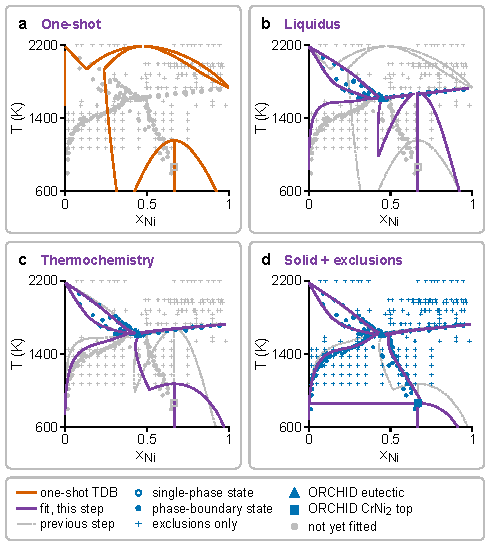
\includegraphics[width=83mm]{fig_crni_sequence_1col}
    \caption{The Cr--Ni fit sequence, from the one-shot model to the final fit, calculated with pycalphad. (a)~The one-shot model of PhaseForge, without any fit. (b)~After the liquid step, fitted to the liquid phase-boundary data, the eutectic and the excess entropy of the liquid. (c)~After the thermochemical step, with CrNi$_2$ free. (d)~The final fit, with the solid-state data and the excluded phases at every observed state. Purple lines: the current step; dashed grey: the previous step. Markers: the 695 experimental states, in blue where the current step uses them and in grey where it does not yet. ORCHID v2026.10 and records extracted for this work; record identifiers are provided with the source data.}
    \label{fig:sequence}
\end{figure}

In the second step, we add the thermochemical data to the fit, with CrNi$_2$ free but anchored to its one-shot energy via an observation with its uncertainty. The effect of this step is to lower the top of the compound to \qty{1074}{\K}, while the lowest temperature of the liquid remains at \qty{1626}{\K} (\cref{fig:sequence}c). In the last step, we add the phase-boundary data, along with the excluded phases at all observed states, and adjust the model's solid-state boundaries to the evidence. The resulting model places the eutectic at \qty{1614}{\K}, compared with \qty{1618}{\K} in the ORCHID record (with an effective uncertainty of \qty{11}{\K}), and the top of CrNi$_2$ at \qty{860}{\K}, compared with \qty{863}{\K} (\qty{16}{\K}) in a record that has so far been read by a single reader (\cref{fig:sequence}d). At each step, the model changed mainly in the region the newly added data could constrain: first in the liquid, then in the compound and the thermochemistry, and finally in the boundaries of the solid state, which is precisely the purpose of a sequence like this.

Two invariant temperatures are not enough to judge a phase diagram, and for this reason the final model was also compared with each of the 695 experimental states in the evidence bundle. For 599 of these states, the phases calculated at the reported temperature and composition include those observed; for 424, the calculated and observed assemblages are identical, while an excluded phase appears as stable in only 6 states. However, the extent to which a state is reproduced depends on how completely it was characterized in the original work. Complete tie-lines, for which both phases and both compositions are known, are reproduced in 40 of 41 cases, whereas this is the case for only 306 of the 489 single-phase states and 78 of the 164 partial tie-lines. In part, this difference is a consequence of the comparison itself. Since each state is evaluated at its reported coordinates and not within its uncertainty, a point close to a calculated boundary can easily fall on the wrong side of it, and these counts should be read as a lower bound of the agreement. For the thermochemical data, in contrast, the agreement is of the order of the reported uncertainties, with root-mean-square standardized residuals of 1.22 for the 113 activities and of 1.05 for the 130 enthalpies.

However, not all mismatches result from the comparison, and the largest ones in fact point to a real limitation of the model on the Cr-rich side of the diagram. According to the final model, sixteen single-phase bcc states reported in three independent studies~\cite{svechnikov1962characteristics,dench1963adiabatic,collins1988electron} lie inside the bcc + fcc or bcc + liquid fields. This means that the model places the boundary of the bcc solid solution at higher Cr contents than those observed (up to 0.088 in mole fraction at \qty{1403}{\K}, and 0.045 to 0.07 between \qty{1650}{\K} and \qty{1822}{\K}), that is, at four to eight times the uncertainty of the states. The same discrepancy appears in the residuals of these datasets, which are the largest of the fit. On the fcc side, on the other hand, it is the evidence itself that is inconsistent. Three fcc states reported by Jette et al.~\cite{jette1934xray} at $x_{\mathrm{Cr}} \approx 0.55$ and about \qty{1380}{\K} lie well beyond the fcc boundary of the model, while the fcc states of two other studies~\cite{collins1988electron,hao2021}
 at $x_{\mathrm{Cr}} = 0.40$--0.49 agree with it. We do not attempt to decide between these sources. However, both discrepancies are recorded in the assessment and point to the region of the diagram in which new measurements would be most useful.

\begin{figure*}[tb]
    \centering
    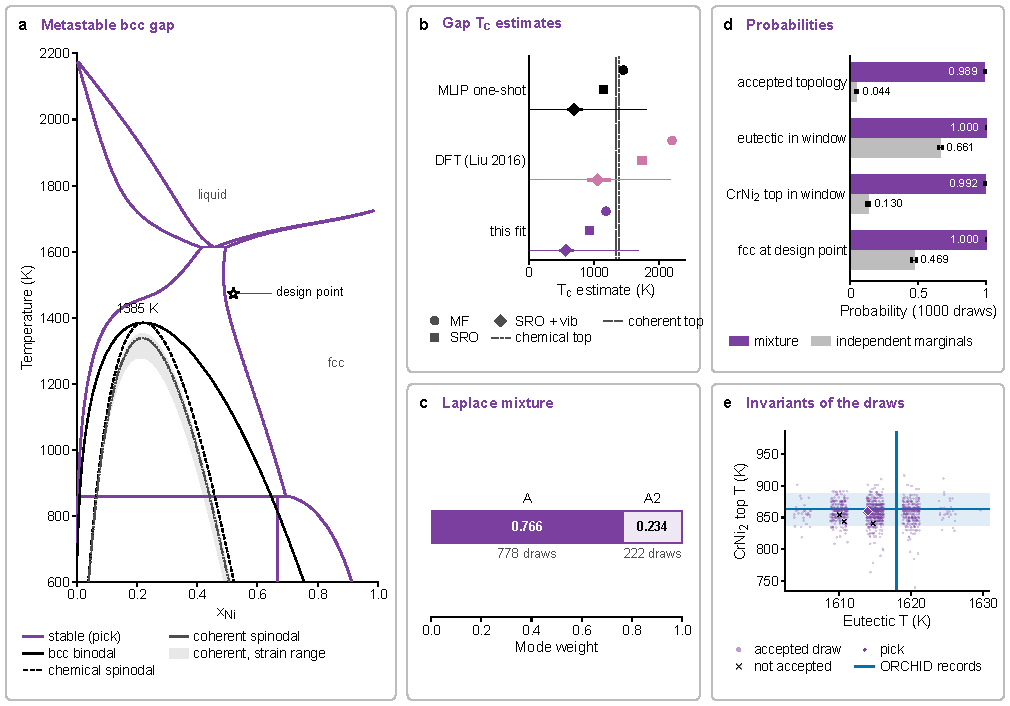
\includegraphics[width=171mm]{fig_crni_physics_uq}
    \caption{Physics and uncertainty of the final fit. (a)~Stable diagram (purple) with the metastable miscibility gap of BCC\_A2: binodal, chemical spinodal and coherent spinodal (grey band, range of coherency strain energies), all inside the stable two-phase fields; star, the design point at $x_{\mathrm{Ni}} = 0.52$ and \qty{1473}{\K}. (b)~Estimates of the critical temperature of the bcc gap as a regular solution, with short-range order and with the excess vibrational entropy, for the one-shot model, the DFT values of Liu et al.~\cite{liu2016alcocrni} and the fit. (c)~Weights of the two modes in the Laplace mixture. (d)~Probabilities of the accepted topology, the eutectic and CrNi$_2$ ranges and single-phase fcc at the design point, from the mixture (purple) and from independent marginals (grey). (e)~Eutectic and CrNi$_2$-top temperatures of the 1000 draws, with the ORCHID records (blue) and the final fit (diamond). ORCHID v2026.10 and records extracted for this work; record identifiers are provided with the source data.}
    \label{fig:physics}
\end{figure*}

The final model passes the physical checks described in \cref{sec:methods:checks}. The pure elements reproduce the SGTE descriptions, with bcc Cr and fcc Ni stable below their melting points, the liquid is convex in composition at all temperatures between \qty{600}{\K} and \qty{2200}{\K}, and no stable miscibility gap appears in either of the solid solutions. These checks also reveal a feature of the model that is not visible in the phase diagram: a metastable miscibility gap in the bcc solution. The chemical spinodal of this gap reaches \qty{1385}{\K} at $x_{\mathrm{Ni}} = 0.22$, and the elastic term of Cahn lowers the coherent spinodal to \qty{1338}{\K} (\cref{fig:physics}). Since the gap lies inside the bcc + fcc field, where fcc is the stable phase, it cannot be observed in equilibrium. The question of whether such a gap is reasonable cannot be settled with the energetics of the potential either. When short-range order and the excess vibrational entropy are taken into account, the incoherent estimate of the critical temperature obtained from the energetics of the potential is about \qty{700}{\K}, but the uncertainty of this estimate, which follows from the error of the potential, extends from zero to about \qty{1800}{\K}. Following \cref{sec:methods:checks}, we left the gap to the data, so its position in the final model is determined by the evidence rather than by one-shot energetics.

In order to estimate the uncertainty of the final model, the two modes of the flat basin were combined into a Laplace mixture, in which they enter with weights of 0.77 and 0.23, and 1000 parameter vectors drawn from this mixture were classified according to the procedure of \cref{sec:methods:uq}. It is important to note that 98.9\% of these draws give the accepted topology, while the eutectic remains within \qty{1610}{\K} to \qty{1620}{\K} and the top of CrNi$_2$ within \qty{830}{\K} to \qty{885}{\K} with a probability of 90\% (\cref{fig:physics}). This means the parameters left undetermined by the evidence have little effect on the model's predictions, consistent with the agreement between the two modes discussed in \cref{sec:reproduction}. This conclusion, however, depends on the correlations between the parameters. When the same marginal distributions are sampled independently, only 4.4\% of the draws give the accepted topology, and the top of CrNi$_2$ is spread over more than \qty{1000}{\K}. The Hessian-described correlations are thus an essential part of the uncertainty in a CALPHAD model, to the extent that neglecting them would grossly overestimate the uncertainty of the phase diagram.

\subsection{Discussion}
\label{sec:discussion}

The level of reproducibility demonstrated here has a cost, and it is therefore important to consider what is gained in exchange for it. Most of this cost is associated with the preparation of the record, which involves writing the general protocol, assembling the evidence together with its uncertainties and excluded phases, and documenting each run and each decision as the assessment proceeds. In this work, AI agents carried out much of this effort under the protocol, and the assessor's additional work was limited to the decisions the protocol reserves for people. In contrast, the cost of using the record once it exists is small. The complete regeneration of the Cr--Ni assessment by an AI agent through the server required 2~h~38~min on a single workstation, at a cost of US\$1.64 in model usage. In exchange for this cost, it becomes possible to verify any number in the database against the evidence and the decisions from which it originated, to detect errors in the record itself (as happened twice in the course of this work) and to extend the assessment as new data become available, without the need to reconstruct it from the beginning.

Some parts of an assessment, however, resist exact reproduction, and it is for these parts that the distinction between the kinds of steps of a protocol becomes important. Relaxations and molecular dynamics simulations performed with machine-learned potentials on GPUs are not bitwise deterministic, and an optimizer's trajectory depends on processor architecture, as shown by the different proportions at which the Cr--Ni fit reached its two modes on the two machines. For such steps, the standard requires agreement within tolerances that are declared in advance and based on the spread observed between repeated runs. A check of the liquid simulations on two DGX Sparks shows why the spread has to be measured rather than assumed. Runs started with the same seed did not reproduce their volumes even on the same GPU, and when the volume of the cell was averaged over only \qty{5}{\ps}, the enthalpies of the individual states differed between the two machines by up to \qty{3.5}{\kilo\joule\per\mole} of atoms, which is considerably more than their statistical errors would suggest. With an averaging window of \qty{50}{\ps}, in contrast, every state agreed to within twice its standard error. The enthalpy of mixing of the equiatomic liquid agreed between the machines within this tolerance for all three windows, with values between $-2.3$ and \qty{-4.4}{\kilo\joule\per\mole} of atoms compared with \qty{-3.2}{\kilo\joule\per\mole} of atoms in the assessment, and this spread remains well below the uncertainty of \qty{9.7}{\kilo\joule\per\mole} of atoms that is assigned to these values in the fit. In the case of the fit, these tolerances apply to the predictions of the model rather than to its parameters, because parameters in the nearly flat directions of the objective can change considerably with no effect on the phase diagram. An important consequence of this choice is that two assessments are regarded as equivalent when they predict the same phase diagram and thermochemistry, even when their parameters differ. The parameters that the evidence leaves undetermined, in turn, are reported as such, instead of being presented as quantities known to the precision with which they are printed.

A related question is why the protocols of ORCHID-SAGE were not written in an existing workflow language, such as CWL~\cite{crusoe2022cwl}. The reason is that a CALPHAD assessment is only partly a computation. A large fraction of its steps consists of judgments (the choice of phases and models, the acceptance of records, the selection of a fit among several candidates), while other steps require GPUs or campaign-specific code that a workflow engine would not run in a portable way. For this reason, the protocols record the assessment plan and the decisions taken along it, and refer to the exact command and code that were used for each executable step. This design does not exclude a workflow language, however. The deterministic and numerical steps of a specific protocol could be exported to CWL and executed by any compliant engine, with the judgment steps supplied from the decision log, and such an export would make the standard compatible with the infrastructure for workflows that already exists in other fields.

A complete record also brings to light questions about the model that would otherwise go unnoticed, and the metastable bcc gap described in \cref{sec:crni} is a case in point. In the final model, the chemical spinodal of this gap reaches \qty{1385}{\K}. The incoherent estimate of the critical temperature obtained from the fitted interaction parameter of bcc, in contrast to the one obtained from the energetics of the potential, and corrected for short-range order and for the excess vibrational entropy, is close to \qty{570}{\K}. The experimental data therefore imply a considerably larger gap in the model than the corrected energetics suggest. The information contained in the present record is not sufficient to explain this difference, and we do not attempt to explain it here. The point to be made is rather that such a difference can only be identified when the energetics, the corrections and the fitted parameters are part of a single record, and when the rule according to which the gap was left to the data has been stated before the fit was carried out.

The Cr--Ni assessment is, of course, only a first test of the standard. Binary systems with ordered phases, with compounds of wide homogeneity range or with magnetic contributions, as well as ternary systems in which several binary descriptions have to be combined, will place demands on the general protocol that the present case did not, and we expect the protocol to grow, version by version, as these systems are assessed. The evidence is not in its final form either. Some of the data used in this work were extracted by a single reader and are not yet part of a released version of ORCHID, so that they remain flagged in the assessment until a second reading confirms them. The reproduction reported here, finally, starts from the one-shot energetics, since the calculations with the machine-learned potential were only checked for a small sample of structures on a second GPU. A full regeneration of these calculations is possible with the same protocol, although it would take considerably more computing time than the rest of the assessment.

Beyond these limitations, the most important consequence of a standard of this kind is that \emph{it allows a thermodynamic database to take part in the loop between prediction and experiment} described in the \textbf{Introduction}. A database that can be regenerated from its record can also be updated when new evidence appears, by adding the new observations to the evidence bundle and running the specific protocol again, with every decision that is not affected by the new data kept as it was. In a self-driving laboratory~\cite{abolhasani2023selfdriving,szymanski2023alab}, the phase stability predicted by such a database, together with its propagated uncertainty, can guide the choice of the next experiments, and the observations made in these experiments can be recorded in ORCHID as fully defined thermodynamic states and used to refine the database. 

Since an \textbf{AI agent can carry out the refinement} through the server, each version of this living database remains traceable to the evidence and the decisions from which it was obtained. The Cr--Ni assessment reported here is a first step in this direction, and the Cr-rich region of the bcc solid solution identified in \cref{sec:crni}, where the model and evidence disagree, is precisely the kind of place to which such a laboratory would direct its next experiments.

